\documentclass[a4paper]{article}
\usepackage{a4wide}
\usepackage{fancyhdr, graphicx}
% Voir https://stackoverflow.com/questions/544907/remove-boxes-from-hyperlinked-toc-in-latex
\usepackage[hidelinks]{hyperref}
%
\usepackage[utf8]{inputenc}
\usepackage{xspace}
\let\OldTexttrademark\texttrademark
\renewcommand{\texttrademark}{\OldTexttrademark\xspace}%
\renewcommand{\headrulewidth}{0pt}
\fancyhead[R]{}
\fancyhead[L]{

\includegraphics[width=1.5cm]{logo_chainons_noirs.png}
}
\fancyhead[C]{

\includegraphics[width=6.5cm]{logo_sesame_noir.png}
}
%\hypersetup{%
%    pdfborder = {0 0 0}
%}
\newcommand{\version}{\vspace{10pt}\\ Version 1.1}
\newcommand{\smallvspace}{\vspace{4pt} \\}
\begin{document}
\title{Whitepaper \vspace{10pt} \\
\large For a 3-click Web3 certified AML~\footnote{Anti-Money Laundering}}
\author{Cyril Chad\'e, Thomas Guerber and Christophe Ramananjaona}
\date{\today\version}
\maketitle
\thispagestyle{fancy}
\tableofcontents
\newpage
\section{Introduction}

The adoption of blockchain technology by a rapidly growing number of industries, and the rapid increase of proliferation of crypto assets as a permanent part of the financial landscape, as well as in the entertainment, art, insurance, gaming, shopping, logistics and real estate, makes the case for an increase of regulatory pressure and the need for safety and compliance tools. Throughout the world, legislative bodies have been pushing for stricter rules regarding the identification of the parties involved in cryptocurrencies purchases, trading, marketing operations, offerings of complex financial products, and the tracking of funds.
However, by its own definition, a cryptocurrency ecosystem, tends to hide the real identity of the transacting parties, as blockchain technology is based on distributed ledgers, cryptography, and pseudonymity. This contradicts the regulating authorities’ mission to counteract illegal activities, such as scams, money laundering, or terrorist financing. As a result, the web3 ecosystem might still appear deeply inadequate in offering the society at large a system which is safe, fair, and trustworthy. 
Most of the crypto industry now agrees on the need for more compliance, transparency, and legality to foster mass adoption and accommodate billions of new users. A direct consequence of this is that clear visibility over the source of funds is becoming a crucial issue for regulators as well as for businesses and individuals. On public blockchains all transactions are visible, therefore funds tracking is completely feasible, yet time-consuming and often reserved to the technically savvy. \\

We can achieve this, by integrating the analysis of on-chain transactions, the so-called “KYT” or Know Your Transaction (comparable to the TraFi “KYC”), into a smart contract which will keep the users’ wallet in a safe and trustworthy space. \\

By putting technology at the service of regulation we can solve the challenges arising from the continuous innovation in the cryptospace. \\

As a RegTech company, our goal is to progressively create trust areas where financial transactions between certified wallets and certified smart contracts are assertively deemed compliant. Hence, the Web3 community is provided with a secure and safe ecosystem to develop its economy, while still keeping the privacy-protecting and decentralized spirits which are attached to its roots.

\subsection{The Company}
Sesame.fi is a French-based company specializing in crypto compliance certification. We aim to build the next global compliance standard for Web3 and accelerate its adoption by regulated entities and individuals with transparency needs. \\

Our core service is an easy-to-use score-based AML and Know Your Transaction procedure. This service will ensure the certification of wallets and their owners and drive them to Web3 Trusted Spaces where all the peers will transact safely, with no fear of contagion by fraudulent or suspicious activity. \\

With the world’s highest-standard compliance AML providing partners, Web3 teams of experts, and Web3 products partnerships, we are achieving one of the most awaited needs: transparency in the industry.
\subsection{Core Team}
As a French-based fintech startup, we have gathered a team of solid and complementary experts to join forces in various domains and industries, all involved in Web3 and Blockchain for many years, to succeed in this new entrepreneurial journey.

\begin{itemize}
\item 
Christophe Ramananjaona \smallvspace
PhD geophysicist \& high-performance computing developer with more than 20 years of expertise in data processing and numerical models for academia and the oil and gas industry with a keen interest in smart contracts and leveraging blockchain technology.

\item 
Cyril Chadé \smallvspace
Entrepreneur, investor \& government advisor created 4 companies in Web1, Web2 \& Web3, and successfully exited 2 of them. Advisor to European governments, ministers, law-makers, and institutions. Advisor of numerous tech companies: Google, Facebook, Lime. 

\item 
Thomas Guerber \smallvspace
Crypto investor since 2012. Law and Finance professional. Journalist, copywriter and builder in the blockchain space. French Financial Market Authority Certification (AMF)
\end{itemize}

\subsection{The issues}
As blockchain and digital assets become more widely adopted and regulated, banks and financial institutions, as well as luxury brands, artists, auctions, real estate, medical researchers, logisticians, and many more want to enter the decentralized world with as much guarantee as possible to:

\begin{itemize}
\item Buy and Sell digital assets
\item Fulfill the needs of their customers
\item Take advantage of some decentralized finance products
\item Build their own services and applications in a distributed ledger
\item Inter-operate using a more secure, transparent and efficient technology
\end{itemize}

These actors are more and more vigilant with regards to the directions the market is taking, and the decisions that governments take with regards to regulating the use of cryptocurrencies. At the same time, they are willing to adopt common standards to allow mass adoption. \\

Individuals use Web3 products (DEXs, NFT marketplaces, etc.) without knowing the counterpart they are dealing with. These decentralized exchanges, NFT marketplaces, or liquidity pools do not check the origin of funds which transit through their services, and this origin remains consequently unchecked, as it is  one of the core values of Web3 to preserve pseudonymity by not revealing the true identity of a wallet owner. The current structure of the Web3 industry deters large financial actors and other compliant bodies like non-profit organizations from participating in this industry. Billions of dollars are thus missing in the ecosystem, due to a lack of guarantees and compliance. \\

The following questions then arise: 

\begin{itemize}
\item[-] {\it How do we clearly identify malicious actors inside Web3 products and put them aside?}

\item[-] {\it What kind of mechanism can we set up to create a risk-less space for legit actors and at the same time preserve their pseudonymity?}
\end{itemize}

The recent U.S sanctions on the Tornado Cash mixer and the subsequent blacklisting of all the addresses linked to Tornado Cash by several Web3 services is a perfect illustration of the regulatory attempt at limiting the circulation of fraudulent assets. This blacklisting has been implemented in the form of an end-point which would be called by the application front-end. However, users quickly found ways to circumvent the restriction by either spinning out a complete fork of the front-end service they wanted to access, or adding a new extension to their browser which would trick the actual front-end application by providing it with a fake compliant response.
It then becomes obvious that the compliance checks need to be applied on-chain. \\


This where how Sesame.fi wishes to address these questions.
\subsection{The solution}
By pushing the compliance tools on-chain, Sesame.fi aims to accelerate cryptocurrencies adoption by providing maximal reliability and transparency for all Web3 users. Our RegTech solution is to provide an easy-to-use interface which will certify whether a wallet is compliant to a specific compliance standard or not. This interface will come in the form of an on-chain whitelist. \\

In theory, anyone, whether it is an individual, a business or an institution can check any wallet, track its transaction history and make sure it has never dealt with litigious funds. However, this task is tedious and often reserved to the realm of AML providers. \\

Sesame aims to use the results by these AML providers to summarize their analyses in a concise, user-friendly form that will be readily usable to perform quick background checks on transacting wallets. After deciding on a reasonable threshold of compliance, those compliant wallet addresses will be stored on-chain, and verifiable from anywhere through the whitelist smart contract interface. \\

By maintaining a real-time, global whitelist of positively compliant addresses, and checking those with which they are interacting, we can open new possibilities for the Web3 space, and create a more secure environment. Ensuring these wallets can transact in Certified Trust Spaces\texttrademark with tested peers. \\

As a direct answer to regulatory pressure that is coming, the standard of compliance which Sesame envisions is higher than the current banking standards. Being associated with a series of AML providers, each test will be conducted by at least 3 of them, and up to 8 high-quality KYT providers. \\

Through the mastery of decentralized web technologies, Sesame will provide a certification that will guarantee, in real-time, that millions of blockchain participants can transact without worrying about the risks associated with the origin of funds of their counterpart. By leveraging on-chain smart contract technologies, we can guarantee the transparency of the system and the compliance of all the registered addresses, while achieving a high level of resiliency. \\

We are proud to introduce the Sesame Certificate, the digital compliance certificate, will allow users to access Certified Trust Spaces\texttrademark in Web3. These spaces will be on-chain spaces only accessible to certified wallets, thanks to the implementation of an on-chain background check. The simplicity of this background check, which will result in a green light/red light response, will keep the user experience seamless on the application side, and at the same time free from the worries on compliance issues, thanks to the guarantees brought onto the Certified Trust Spaces\texttrademark users.
\subsection{Advisors}
We strongly believe in collective strength, mutual learning and team synergies. Blockchain technologies are based on mathematics before being an ecosystem, it is a technology and now a business. We surround ourselves with people with the highest theoretical and practical experience in the blockchain industry, as well as the legal and governmental sectors, to build and deploy these new tools and services, from a compliance standard to safe spaces and on-chain certifications. This is why we gather experts with different profiles to build a complementary group. \\

With this in mind, we have created 3 groups of experts: 

\begin{enumerate}
\item Tech: The first group focused on research, and technology, coming from world-class universities and laboratories. These experts will provide us with technical support in building and implementing the on-chain and off-chain solutions.

\item Legal: The second one focused on compliance, legal, governmental relations, public affairs and regulations on an international scale. The purpose of the first group is to accompany us on the legal part in connection with Web3, its ecosystem, and the current changing regulations.

\item Entrepreneurship: Last but not least, we will benefit from the help, vision, and knowledge of tier-one entrepreneurs, creating opportunities, and challenging our goals and vision.
\end{enumerate}

Thanks to this tailor-made support, our compliance standard is ready to become the universal certification that the ecosystem needs.

\subsection{Partners}
Sesame works with key players, movers, and shakers of the digital asset ecosystems, in particular anti-money laundering (AML) providers, world-class engineers, and leading legal experts. Together we aim at providing regulated entities and each and every individual with a single query that will aggregate and verify the data from a wallet using all the providers available, hence reducing operational and compliance risks associated with using only one provider.

\subsubsection{AML Tech companies}
We have a selection of key players in the ecosystem, such as Merkle Science, Scorechain, Crystal Blockchain, BIG, Chainalysis, etc, and we are happy to reach partnerships and trust with the most performing ones.

\subsubsection{Law firms and Compliance Officer}
Compliance Officers became a key element of any worthy crypto company. On the external side of compliance, law firms always play a crucial role in helping nascent technologies keep up with the regulatory updates. Both those actors are natural partners for Sesame. The industry faces a time of construction and innovation where conversation, and interaction within and outside of the ecosystem is key to success.


\newpage
\section{SESAME: The first-ever crypto compliance certificate}
\subsection{Introduction : the principles of KYT}
We are proud to introduce the Sesame Certificate: the digital compliance certificate used to create Certified Trust Spaces\texttrademark in Web3. \\

By doing KYT in real-time on all our clients’ addresses, checking any address and its interactions, we guarantee our users access compliant spaces in DeFi, NFT Marketplace, Metaverse, or any Web3 products, places where one will be sure to interact with safe counterparts and maintain a clean wallet.

\subsection{SESAME v1.0}
\subsubsection{Wallet compliance}
Our simple interface gives any user the possibility to obtain a certificate in less than 2 minutes. In the back-end, we perform queries to a series of AML partners to verify the legitimacy of the address. Statistical and legal analyses will be performed to decide on the proper way to aggregate the various scoring results from the different AML provider, and set the threshold separating a compliant wallet from a non-compliant one.   \\

After validation of compliance, the address will immediately be whitelisted in the Sesame smart contract. The presence of an address in the whitelist smart contract has the validity of a certificate, reflecting that the analysis that the users' funds have not been subject to illicit activities, and works as a passport. This certification is valid for a limited period (initially a 90-day validity) and will require renewal after this period. Conversely, a user staking a defined amount of our utility Sesame tokens will benefit from the service as long as the right amount of tokens remains staked in the staking smart contract. \\

This service is accessible to anyone, both institutional actors and retail investors can check the source of their assets. Scoring an address only costs a few dollars which gives universal access to a necessary service which is currently only available to governments and big players. The first version of the Sesame solution will focus on the Ethereum blockchain to maximize the Web3 ecosystem impact, but the longer term solution will be applied to multiple blockchains. At the moment, the technology stack will allow a user to score any Ethereum address and pay from any Ethereum compatible blockchain, such as Binance Smart Chain, Polygon PoS, Avalanche C-chain, etc, while we handle all the whitelist operations from the Ethereum blockchain. 

\subsubsection{Real-time monitoring of all transactions to ensure Certified Trust Space\texttrademark stability} 
A monitoring service checks in real-time all the scores associated with a certified wallet counterpart address whenever the former transacts on the blockchain, and updates the whitelist according to the scoring result of the counterpart, block after block. \\

Every time a transaction involves a whitelisted address, the monitoring tool detects it and automatically renews the scoring to check if the address is still respecting the chosen standard. If not, the address is removed from the whitelist and its passport is invalidated. \\

The tool will work for all the blockchain tokens monitored by the AML partners, which could represent several thousands of tokens and a large number  of Blockchains.
\subsection{Multi-Chain compatibility} 
Leveraging the technology of our AML providers, we can explore the transactions of more than 25 blockchains to create Certified Trust Spaces\OldTexttrademark. We plan to invest in the Ethereum blockchain first, before looking into the other EVM-compatible blockchains, like Tron, Binance Smart chain, Ethereum Classic, Avalanche, and Layer 2 chains. Then, we’ll open our tool to non-EVM compatible blockchains (Bitcoin, Cardano, Solana, Algorand, etc.). For more details about Sesame deployment see the Roadmap section. 

\subsection{Building a universal standard} 
\subsubsection{Strengths and weaknesses of the Blockchain}
Blockchain has unique characteristics that make it so interesting: it’s pseudonymous, transparent, decentralized or more précisely distributed, and secure. Its very principle is that anyone can interact with anyone, without intermediation, but therefore also possibly without the guarantees provided by intermediaries. Trust is ensured by its intrinsic mechanisms, particularly on a macro scale, through consensus. Last but not least, blockchain is also entirely traceable and the entire history of transactions can be read and checked in the blocks. \\

Those characteristics brought tremendous innovation but also revealed some drawbacks.  The rise of cryptocurrencies was quickly followed by the birth of a thriving black market ecosystem on the web, capitalizing on the strength of blockchain technologies. Even though law enforcement has stopped the vast majority of those activities, a significant portion of crypto transactions is used to launder proceeds from real-world criminal activities. Lastly, with the advent of DeFi, hackers have been relentlessly abusing the flaws in the protocol setups and codes to steal millions of dollars. We strictly reject the reputation of cryptocurrencies being less compliant than any other financial instrument; like traditional finance also has its negative aspects. Nevertheless, we have, by the nature of this technology itself, the means to reduce these negative effects, which is the purpose of Sesame.

\subsection{Gather lawful users}
Sesame intends to create Trust Spaces through Web3, to marginalize bad actors and tame crypto assets. In time, our Certified Trust Spaces\texttrademark will grow, as more and more users and projects will comply with the nascent crypto regulations. In the end, a vast majority of crypto markets will become safe spaces filled with lawful users and legit transactions.  \\

Sesame builds its services on the strength of blockchain technology, legal knowledge and statistical analysis to create a universal standard for KYT and a fully transparent, pseudonymous, and secure passport to enter those Certified Trust Spaces\OldTexttrademark. It’s time for a universally accessible distributed and privacy respectful but at the same time safe and secure transaction system. This standard will be built by setting parameters of AML on the best international standards of financial compliance. 

\subsection{Certified Trust Space\texttrademark label}
\subsubsection{Web3 partners can welcome compliant-only users in dedicated areas}
During the first stage of the project, Web3 projects will be able to use our Certified Trust Space\texttrademark label at no cost, given that they fulfill the best practice requirements of the Certified Trust Space\texttrademark specifications. Any Web3 project dealing with crypto-assets can claim the Certified Trust Space\texttrademark label. Thanks to this label, the users holding the Sesame Passport, will be able to use these Web3 services and be sure they interact only with compliant counterparts within these Trust Spaces.

\subsubsection{Web3 services will adapt their filters to their local legal obligations}
In a second stage, the Certified Trust Space gateway can allow tailor-made filtering of the users depending on the local requirements and jurisdiction. For example, depending on the jurisdiction, specific types of activities are forbidden, like casino and gambling tokens in South Korea. Partners wishing to opt for this kind of solution will be able to get support from Sesame to define the settings of the AML score aggregation and will de facto use a specific whitelist, representative of their affiliated jurisdiction (i.e. ban on gambling-related tokens in Korea, upcoming MiCa regulation in Europe, etc.).

\subsubsection{User centric advantages in Certified Trust Spaces\texttrademark} 
Lastly, the Certified Trust Spaces\texttrademark will need to bring some advantages to the users taking the compliant way. Those advantages might be materialized as priority access to new services or advanced features or extra staking and yielding rewards. We can even think of companies allowing only Sesame-certified users access to services like an auction, a marketplace, etc. The idea is simple: compliance should and will be rewarded.

\subsection{Additional revenue streams}
\subsubsection{Bridging the gap between Web3 and compliance}
We will also be offering a Legal Consultancy Service that can advise any Web3 owner on the latest rules in terms of crypto compliance and the way how they can fulfill the requirements enforced by law, depending on the jurisdictions where they have established their activities. \\

Partnerships with law firms and law professionals can help integrate our Certified Trust Space\texttrademark into the majority of Web3 projects smoothly and help reduce the regulatory risks globally and locally.

\subsubsection{Premium services}
From shrimp, to fishes, sharks and whales, everyone will be welcome to score their various wallet addresses at a fixed price. Whenever a scored wallet comes out with a significant amount of crypto, the owner will have access to a different user experience and an opportunity to subscribe to extra services designed to cater to his or her specific needs. \\

For this type of high-value wallet, we offer a range of compliance and intermediary services for a fee of 0.1\% of the value of the wallet.
\subsubsection{Institutional Scoring} 
Sesame aims to create a safer and more compliant Web3 at minimal cost for the public but it is also able to adapt its solution to the needs of financial institutions. 
For instance, a wealth manager launching a new crypto service for its client base could benefit from our scoring capacities to make sure his clients’ funds are compliant with their jurisdiction regulation, before accepting to manage their crypto assets. \\

Then, each time new clients want to enter the service or add new crypto funds to their portfolio under management a scoring can happen. For this part of the business, we offer both on-chain and off-chain scoring depending on what our interlocutor is more comfortable with. 

\newpage
\section{The Sesame (SAM) token}
\subsection{Utility}
The Sesame token (SAM) main purpose is to unlock unlimited access to Sesame solutions. Initially, users will need to stack 60 SAM to get unlimited access to our scoring and monitoring service. This should correspond to approximately three years of paying for the service as you go. For stacking users, the main upside is that they can add funds and interact outside of the Certified Web3 Spaces without needing to pay again to make sure their wallet is still compliant. The SAM token will have a fixed supply of 100 million units on the blockchain where it will be launched.
\subsubsection{Claiming a certificate after a successful Scoring} 
For individuals who wish to access a Certified Trust Space\texttrademark must obtain a Sesame Certificate. In order to claim it, every address which wishes to be registered has to pay through the Sesame application front-end to get a score and the passport by entering the whitelist. These funds will be used to ensure the sustainability of the project in its initial stages. In the longer term, the aim is to delegate a number of these services to a DAO, including smart contracts management and token policies, i.e. the number of SAM which need to be stacked to enjoy the free service, to the users community.
\subsubsection{Stacking: access to premium services}
As mentioned before, after every transaction made by a whitelisted address, the compliance has to be refreshed (except if the transaction occurred with another whitelisted address) to make sure the address is still admissible in the Certified Trust Space\OldTexttrademark. Every whitelisted user has to go back to our tool to re-score his address and claim the Sesame Certificate again after every transaction with a non-compliant address. Because transactions can be numerous and most users at some point will not be able to do without our service, any user that stacks 60 SAM will get unlimited access to scoring and automatic renewal of the certificate for his stacking address, 
\subsection{A tailor-made Compliance Certificate} 
At first, any Web3 product will be able to freely integrate the Certified Trust Space\texttrademark label into their products. They can create Certified Trust Space\texttrademark using our open-source repository of smart contract source code, JSON (Javascript Object Notation) and ABI (Application Binary Interface) deployment files, and start to onboard Sesame Certificate owners on their products. Users will have access to any Certified Trust Space\texttrademark product through their certification recorded in our smart contract. This way, all users will be sure that they are joining compliant services, where all participants are also respecting regulations and law and all the exchanged assets are trustworthy.
\subsection{Tokenomics}
\begin{itemize}
\item Token ticker: SAM
\item Token chain: Avalanche C-chain
\item Total Supply: 100,000,000 SAM
\item Initial Circulating Supply: 28,541,667 SAM
\item Initial Market Cap on private sale:  33,333,333 €
\end{itemize}

\subsubsection{Lock-up \& destinations}
\begin{itemize}
\item Private sale Seed: 15\% - Vesting over 24 months after TGE
\item Private sale 2: 10\% - Vesting over 36 months after TGE
\item Launchpad \& IDO fund: 3\% - Fully unlocked on TGE
\item Direct listing liquidity fund: 2\% - Fully unlocked on TGE
\item Team allocation: 10\% - Vesting over 24 months after TGE
\item Advisor allocation: 10\% - Vesting over 24 months after TGE
\item Partnership Fund: 10\% - Vesting over 12 months after TGE
\item Strategic reserve: 10\% - Vesting over 12 months after TGE
\item Token sold for stacking: 25\% - Fully unlocked on TGE
\end{itemize}

\subsubsection{Distribution visuals}
 
\begin{figure}[!h]
\centering
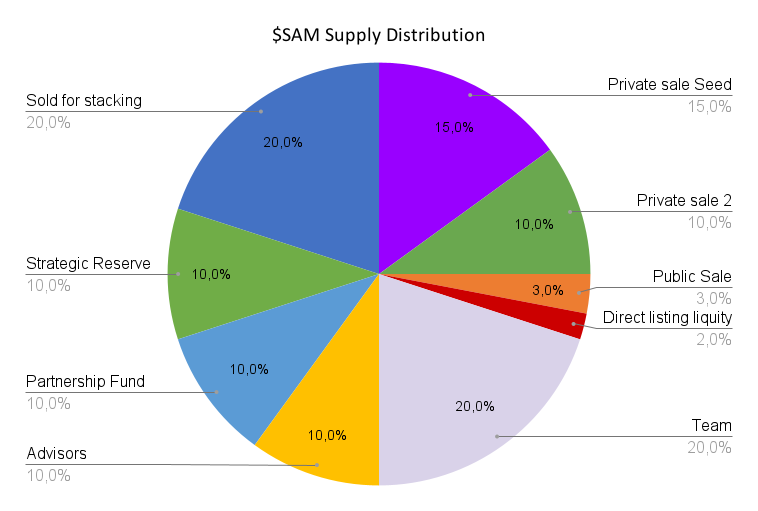
\includegraphics[scale=0.5]{SAM_Supply_Distribution.png}
\end{figure}

\begin{figure}[!h]
\centering
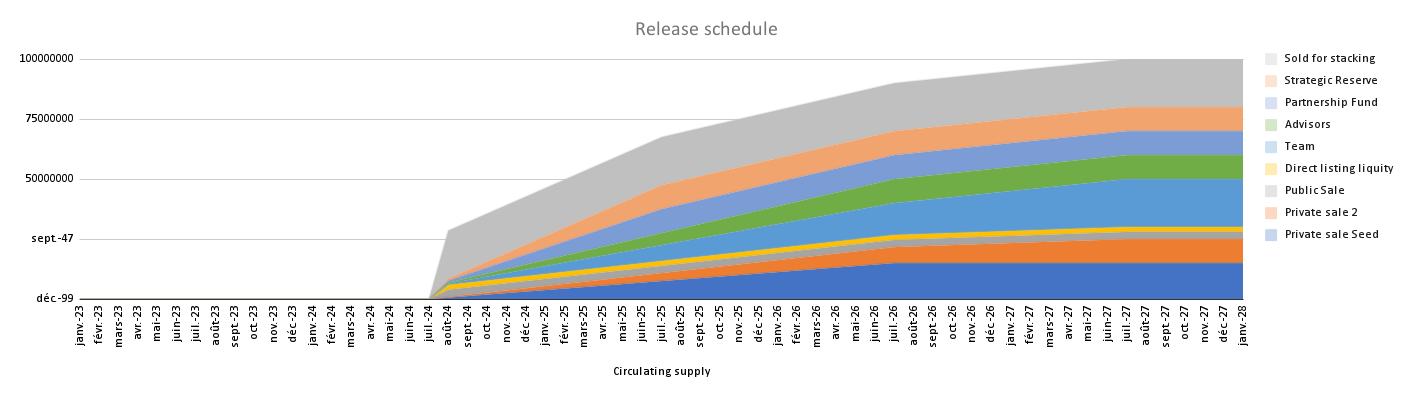
\includegraphics[scale=0.3]{Release_schedule.png}
\end{figure}

\newpage
\section{Customers}
\subsection{Web3 products}
\begin{itemize} 
\item Decentralized Exchanges \smallvspace
Liquidity pools are widespread products of DeFi. Dedicated pools can be very interesting for institutions that want to buy cryptocurrencies for their customers and themselves. For instance, a Certified Trust Space\texttrademark ETH/USDC pool would be a game-changer for a lot of banks and funds to reduce their risks of being used as launderers and ensure compliance of the funds despite the pseudonymity of the participants.

\item 
Launchpads \smallvspace
Launchpads are facing pressure from regulators due to the volume of funds they raise. Several ICOs have been conducted without any KYC or anti-money laundering control. More and more of these providers are willing to add KYC or KYT checks to their platforms, so that they remain compliant to local regulations. A Certified Trust Spaces\texttrademark inside a launchpad will allow them to be compliant with all anti-money laundering regulations. By accepting only Sesame’s whitelisted wallets, these actors will significantly reduce the risk of hosting tainted funds, thus easing the burden of the ever-growing regulatory framework and driving millions of new users to join their platform.

\item 
Wallet providers \smallvspace
A wallet provider would make excellent use of the Certified Trust Space\OldTexttrademark. Integrating our label and onboarding Sesame-scored wallets would reduce the compliance risk for the entity behind the wallet service and allow for the creation of a premium customer base holding only clean coins.

\item 
Blockchain proof of stake validator pools \smallvspace
On a wider scale, we are partnering with whole chains to ensure the compliance of all the assets staked for the Proof of Stake consensus. Scanning wallets, and helping validator projects to create Certified Trust Spaces\texttrademark would in turn help the chains to attract institutions and individual investors thus adding a new dimension to their ecosystem without diminishing any of its added-value or fundamental principles.

\item 
Casinos and Betting platforms \smallvspace
Several high-profile companies are preparing blockchain-based casino and sports betting systems. However, both are often pointed at in the physical world as well as online for helping launder dirty money. By introducing Certified Trust Space\texttrademark into gaming, gambling, and betting platforms, we can imagine a new way for people to interact safely and for these actors to be able to integrate crypto assets in a safe and compliant way.

\item 
NFTs Marketplace \smallvspace
Much like casinos, art is sometimes seen as a way of laundering dirty profits, and the issue is currently creeping on NFT Marketplaces. With the Crypto Trust Space solution, auction houses and NFT marketplaces can create a gateway to allow only Sesame Certificate holders to participate in a sale by excluding tainted coins, thus drastically reducing the risk of money laundering.
\end{itemize}

\subsection{Financial Institutions \& Financial Service Providers}
Diving into the crypto space after years in a given sector is a significant challenge. However, offering crypto services is becoming a necessity for all financial institutions in the coming years. By integrating the Sesame KYT solution to its existing KYC \& AML procedures, any wealth manager or bank will be able to onboard a trove of crypto-holders as clients with minimal risk and an individual scoring for all of their addresses. 
For this part of the Sesame solution, we offer both on-chain and off-chain scoring depending on what the partner financial institution is more comfortable with.

\newpage
\section{Technical Architecture}
\subsection{Door 1.0 (2022)}
The term “door” signifies the gate into the Certified Trust Space. The first release of the solution will include a front-end where a user can pay to register his wallet into the whitelist, given that its aggregated wallet score from various AML providers satisfies the compliance criterion (score below a defined threshold value decided from statistical analysis). \\

The whitelist is an on-chain smart contract managed by the contract owner (the wallet which has deployed the smart contract or the one which has received its custody), meaning that only one wallet is authorized to insert into or remove addresses from it. An off-chain “whitelist manager” micro-service is in charge of this task on behalf of the registration front-end or the monitoring program (see Fig. 1). \\

A copy of the whitelist is stored in an off-chain database to keep a history backup of the whitelisted addresses. A subset of this centralized off-chain database is also serving the requests of the monitoring service to keep the pace of the monitoring program in sync with the creation of new blocks in the chain (the responsiveness of a central database is notably higher than the decentralized smart contract). Regular checks will be carried out to ensure that the database entries match the whitelist entries in the smart contract. \\  

\begin{figure}[!h]
\centering
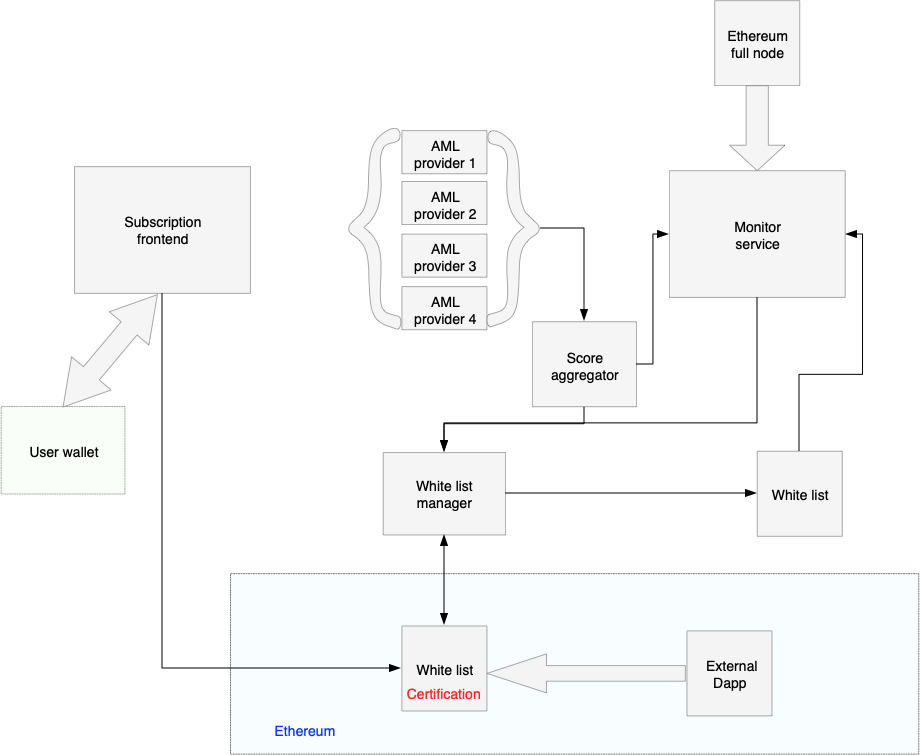
\includegraphics[scale=0.35]{architecture_v1_trim.png}
\caption{Software architecture with off-chain whitelist management}
\label{offchain}
\end{figure}


The monitor program checks every transaction of every block and identifies the addresses which have transferred tokens to the whitelisted addresses, or eventually the one to which tokens have been sent to. If the counterpart address obtains a compliant score from the AML providers, no change is made to the whitelist. On the other hand, if the counterpart address is non-compliant, the whitelisted address is re-tested, and if this last interaction changes its compliance status, the monitor program sends a post request to the whitelist manager to remove the recipient address from the whitelist. \\

Once an address has been registered in the whitelist, the smart contract of a third party DApp can call a function of the whitelist smart contract which will return a “true” boolean value to confirm that the address is indeed compliant, and can then authorize this address to transact in the Certified Trust Space\texttrademark of the Dapp. \\

For the sake of simplicity, the whitelist will be only valid for the blockchain where it has been deployed since decentralized applications will need to make function calls to the whitelist smart contract. However, one of the upcoming features from the AML partners is aggregated scores from different EVM-compatible blockchains for a single address. This means that a score will be identical for a given address on every chain where this address holds tokens, it will be technically possible to make function calls to the whitelist on one blockchain and use the compliance result to authorize or prohibit transactions from that particular address on another blockchain in a decentralized way thanks to the use of a bridge or a decentralized proof of stake transport layer such as Axelar Network (see Figure 2). 
The latter solution will avoid the high gas fees linked to using the Ethereum network. \\

\begin{figure}[!h]
\centering
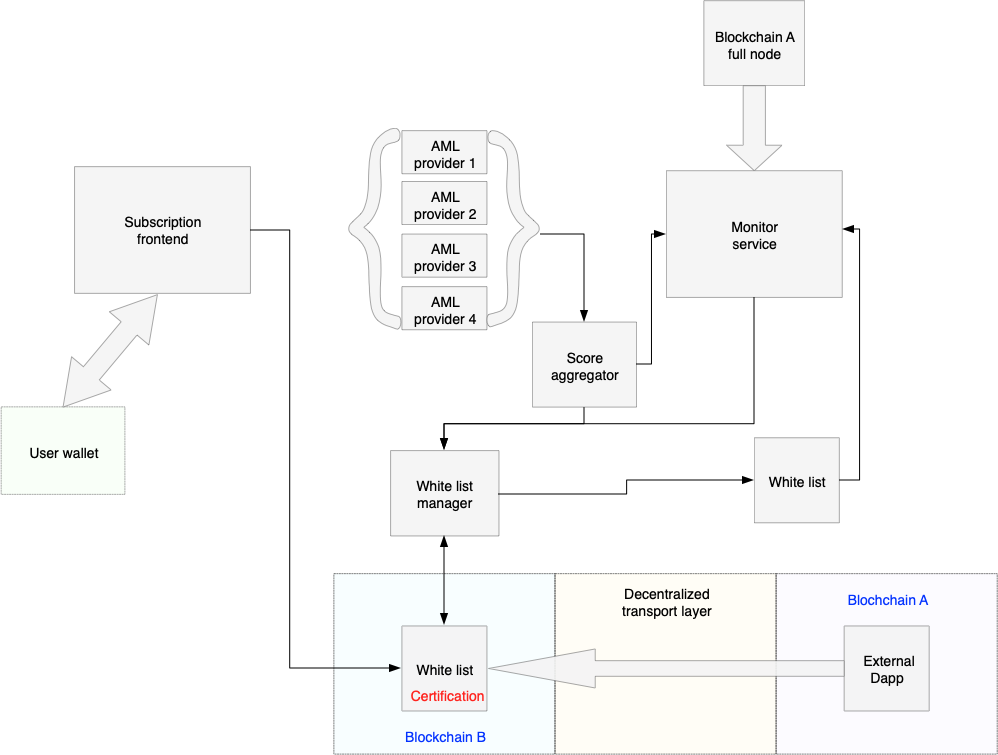
\includegraphics[scale=0.35]{architecture_v1_crosschain_trim.png}
\caption{Software architecture with off-chain whitelist management and cross-chain functionality}
\label{offchain}
\end{figure}  

The compliance status is checked directly in the partner's smart contract by a functional call to the whitelist method deployed on the blockchain. The smart contract Solidity code, its deployment JSON and ABI files will be available on the Sesame GitHub and verified on the blockchain explorer. \\

Partners who wish to access the whitelist from an on-chain function call from a chain which is different from the one where the whitelist has been deployed will make use of the transport layer to route the function call from one blockchain to the other.
\subsection{Door 2.0 (2023)}
The second version of the solution will make use of an oracle to bring the address scoring comparison with the compliance threshold on-chain and will therefore increase the decentralization and transparency of the whitelisting procedure (see Fig. 2). Protection over the free use of the score can then be implemented using encrypted keys which will help prove the confirmation of payment at the front-end side. Oracle providers such as Chainlink or API3 could be used to perform this task. \\  

\begin{figure}[!h]
\centering
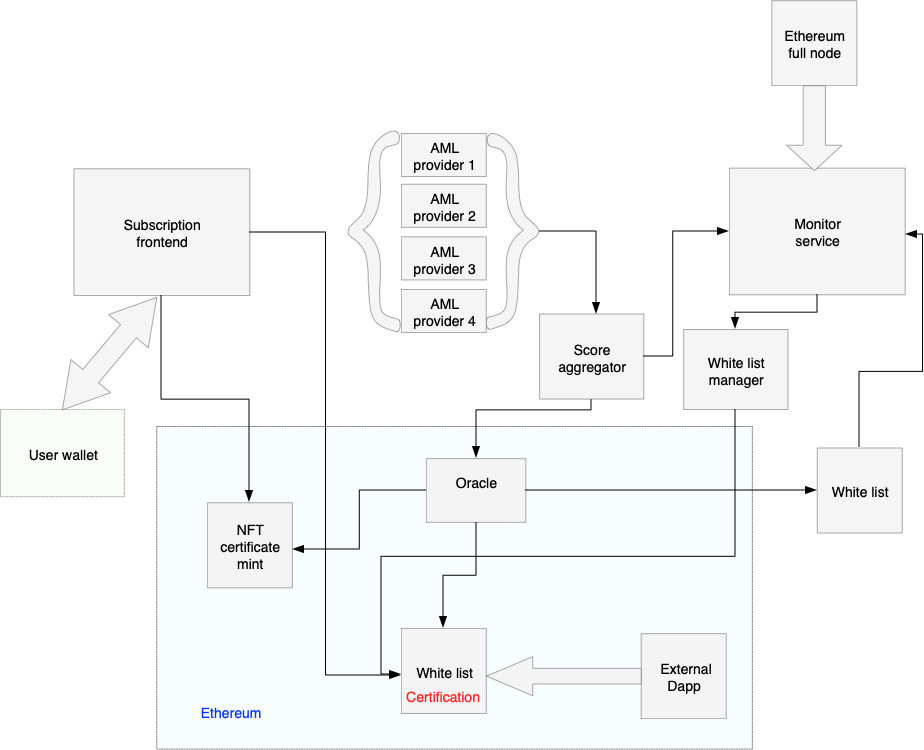
\includegraphics[scale=0.35]{architecture_v2_trim.png}
\caption{Software architecture with on-chain whitelist management and NFT certificate minting}
\label{onchain}
\end{figure}


Again, a transport layer can be used to host the whitelist on one chain and certify the wallets on another one (see Figure 4). \\

The whitelisting technology could also evolve into an NFT passport to be held by compliant users. A separate oracle, an NFT bridge, or the transport layer, could be also used to transfer the passport to another blockchain, as long as the AML providers have aggregated the score of that wallet across several blockchains. \\
  
\begin{figure}[!h]
\centering
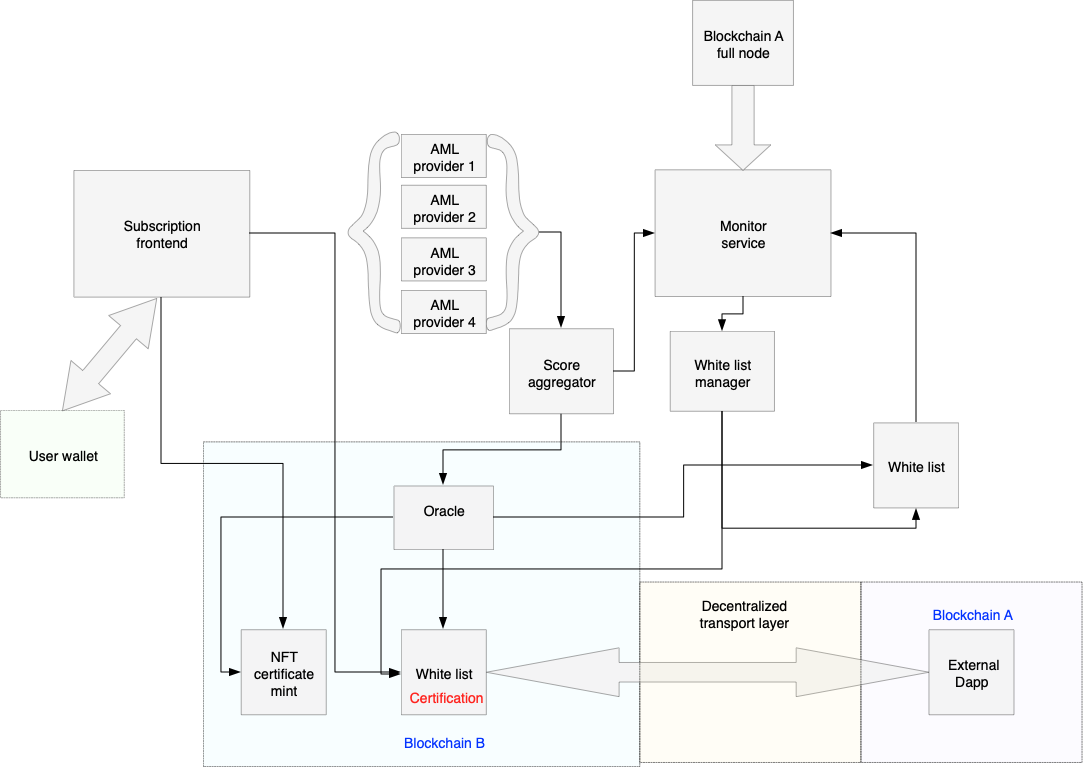
\includegraphics[scale=0.35]{architecture_v2_crosschain_trim.png}
\caption{Software architecture with on-chain whitelist management and NFT certificate minting with cross-chain functionality}
\label{onchain}
\end{figure}


\subsection{Monitoring service}
The monitoring service can be run directly on a local Ethereum full node to maximize the processing speed of every transaction, by not making Remote Call Procedure (RPC) requests through the internet. Multiple nodes might be run to optimize the routes to the various AML providers. \\

At some point, the number of transactions in a block might become so large that a single machine might not be able to process all the transactions of the block before the arrival of the next block. In that case, parallel processing based on Apache Spark will so that transaction verification requests can be made to one node or more. \\

Estimations of the number of wallets to be scored can be assessed by the use of statistical models. In a simplified model where the whitelist registration and churn rates are constant, if one also considers the constant percentage p of wallets transacting every day amongst a total number of wallets $\omega$ , the percentage of wallets registered in the whitelist is given by  

$$S(t)=1-\left(1-S_0\right)\mathrm{e}^{(c-r)t},$$

\noindent where $S_0$ is the percentage number of pre-registered wallets on the whitelist at time $t=0$, $0\le S(t)\le 1$~\footnote{The differential evolution of $S(t)$ is intuitively expressed by $\frac{\mathrm{d}S}{\mathrm{d}t}=(r-c)(1-S)$, and yields the ordinary differential equation $\frac{\mathrm{d}S}{\mathrm{d}t}+(r-c)S=r-c$.}.
Then, the number of addresses for which the score is checked decreases with time as long as the churn rate c is lower than the registration rate r, the number of transactions to track is:

$$\omega p\left[1-S(t)\right]=\omega p\left(1-S_0\right)\mathrm{e}^{(c-r)t}.$$

\subsection{Statistical analysis for determining the compliance score threshold}
AML providers use different systems for scoring the transactions they monitor, and most of the time their system is customizable by the users of their solutions. This is explained in the sense that laws and regulations vary from one country to another. As a consequence, there is no unified international standard for deciding on whether a wallet should be marked as compliant or not. \\

As a first approach, Sesame will aim to certify wallets that comply with the commonly known international law, and will therefore choose parameters that reflect this internationality. \\

Still, a statistical comparison of the scoring results from the different AML providers will be needed to define a coherent score threshold that will reflect the requirement for entering the Certified Trust Space. Mixing and balancing the scores from different providers will be made based on statistical analysis. In this simplified demonstration, we are using the hypothesis that the wallets are uniformly distributed over the AML solutions. The adjustment can be simply made by realigning the mean and the standard deviation of the distribution of scores from the various AML providers with a high degree of redundancy. \\

Since the scores are all between 0 and 1 and tend to be biased towards 1, the assumption is made that the scores provided by each AML report follow a Kumaraswamy distribution, for which the analytical probability density function is given by
$$P(x; a,b)=abx^{a-1}\left(1-x^a\right)^{b-a},$$  

\noindent where $a$ and $b$ are non-negative shape parameter characteristics of the AML provider. This distribution has been chosen for its versatility and its possibly non-symmetric character.
Least-square-type minimization methods such as the conjugate gradient algorithm can then be used to fit the data collected with the AML providers with the theoretical distribution $P(x; a,b)$ so that the parameters $a$ and $b$ can be evaluated. \\

The derivatives used for the gradient vector are
$$\frac{\partial P}{\partial a}=\frac{bx^{a-1}\left(1-x^a\right)^{b-1}\left[a\ln(x)x^ab
-a\ln(x)+x^a-1\right]}{x^a-1}$$
and 
$$\frac{\partial P}{\partial b}=ax^{a-1}\left(1-x^a\right)^{b-1}\left[b\ln(1-x^a)+1\right].$$

For a number of AML providers, the aggregated shape parameters are then given by the average of the individual shape parameters:
$$a=\sum_{i=0}^na_i$$
$$b=\sum_{i=0}^nb_i$$  

More statistical complexity could be added by considering mixtures of Kumaraswamy distributions in order to best approach the actual statistical distribution provided by the AML rating companies, while still keeping the model practical. \\

In the future, the tool could be adapted to local country regulations in such a way that the user could freely choose the legal jurisdiction with which his wallet complies with.

\subsection{Future developments: from NFTzed Passport to private blockchain}
\subsubsection{Privacy}
The privacy of the certificate could also be preserved by using zero-knowledge proofs so that the compliance status is known only by the user and the party to which he agrees to disclose it, i.e. the Web3 partners providing a Certified Trust Space.  The zero-knowledge proof can be implemented for EVM smart contracts using the zk-SNARKs family of algorithms and the alt\_bn128 elliptic curve which are part of EIP-196 and EIP-197. In this case, the wallet address and its score can be encrypted with verification keys and stored on-chain while the proving keys can be kept by the user. In the case of an encrypted whitelist, the compliance status is checked in a similar fashion as without any encryption. \\

Since the cost of registering elliptic curve points on-chain will be much higher than a simple plain wallet address, the encrypted whitelist could be deployed on a niche blockchain, such as Milkomeda Cardano, or even a dedicated Avalanche subnet, so that the gas fees will be close to zero. \\

The case of a decentralized acceptance test combined with the privacy of the scores could also justify the need to run a private blockchain where the actual score aggregation could take place.

\subsubsection{Certificate in the form of a passport}
The certificate could take the form of a passport represented by a non-transferable NFT, or a soulbound token (\href{https://vitalik.ca/general/2022/01/26/soulbound.html}{SBT}). The creation of a standard for SBTs is expected at the end of 2022, therefore it is conceivable to integrate them in version 2.0 of our solution due in 2023. 
Moreover, the use of SBTs will allow the transfer of certificates from one chain to the other. The technology is not completely ready yet at the time of writing, but we can already envisage the use of such solutions to broadcast the certification registered in one unique whitelist to applications on many blockchains. This will greatly simplify the maintenance and consistency of our product.

\subsection{Calls into the whitelist by Web3 partners}
The compliance status is checked on the partner's smart contract or on his website by a functional call to the whitelist method which has been implemented in a smart contract written in Solidity. The smart contract code and its deployment JSON file will be available on the Sesame GitHub.
Partners who wish to access the whitelist from an on-chain function call from a chain that is different from the one where the whitelist has been deployed will make use of an oracle which will make an API call to a service provided on a Sesame node. \\

In the case of an encrypted whitelist, the compliance status is checked in a similar fashion. 

\newpage
\section{Product, company \& token roadmap}

\begin{itemize}
\item
Q4 2022:  v0.1 POC
    \begin{itemize}
    \item EVM-compatible testnets (Kovan, Rinkeby, local, Polygon PoS Mumbai, Avalanche C-Chain Fuji, Milkomeda Cardano, Binance Smart Chain). 
    \item Serial monitor program. 
    \end{itemize}

\item
Q1 2023: v0.2 MVP
    \begin{itemize}
    \item Private beta product launch on testnet and mainnet.
    \item Accepting payments from Ethereum, Binance Smart Chain, Avalanche C-Chain, Polygon PoS, Cronos, Fantom, Arbitrum, Milkomeda, Kava, Aurora, Optimism, Gnosis. 
    \item Free public scoring of EVM-compatible addresses and central database registration.
    \item Parallel monitor program for Ethereum testnet on Spark/Kubernetes.
    \item Audit.
    \end{itemize}

\item
Q2 2023: v1.0
    \begin{itemize}
    \item Official launch of an on-chain whitelist and monitor for Ethereum mainnet.
    \item On-chain registering of the addresses from the central database.
    \item Product without staking. Any user removed from the whitelist needs to subscribe again.
    \item Use of Axelar Network and oracles on EVM-compatible testnets (Ropsten, Polygon PoS Mumbai, Avalanche C-Chain Fuji).
    \end{itemize}

\item
Q3 2023: v1.1
    \begin{itemize}
    \item Official launch of an on-chain whitelist and monitor for Binance Smart Chain and Polygon PoS.
    \item Use of zk-SNARKs on EVM-compatible testnets (Avalanche C-Chain Fuji, etc). 
    \end{itemize}

\item
Q4 2023: v2.0
    \begin{itemize}
    \item Use of Axelar Network for on-chain computation registration of new wallets on Ethereum, Binance Smart Chain, Polygon PoS.
    \item Migration of the whitelist to Avalanche C-chain
    \item Minting of SAM token on Avalanche C-Chain.
    \end{itemize}

\item
Q1 2024: v2.1
    \begin{itemize}
    \item Liquidity pool and staking set up. 
    \item Official launch of a whitelist for Tron.
    \item Token listing.
    \end{itemize}

The whitelist manager checks the address of the staked SAM tokens in the liquidity pool to check if the required tokens are present.

\item
Q2 2024 v2.2
    \begin{itemize}
    \item Official launch of a public whitelist and monitor for Avalanche C-Chain.
    \item Start adaptation to non-EVM chains: Stacks, Ripple, Cosmos, Solana.
    \end{itemize}

\item
Q3 2024 v2.3
    \begin{itemize}
    \item Official launch of a whitelist and monitor for Stacks, Ripple, Cosmos, and Solana.
    \end{itemize}
\end{itemize}

\newpage
\section{Concluding remarks}


The crypto wallet and Web3 project certification are only the first steps for Sesame. Certification as a business model can be declined into a myriad of business lines and various industries by capitalizing on blockchain technology's unique characteristics and crypto innovations. \\

Certification can be applied to environmental, social, or financial considerations as well as respecting some specific set of other criteria like community-based ones. The use of blockchain will lead to a more transparent and secure digital space through the use of decentralized blockchain certification platforms and to the capacity of each and every user to use and benefit from this revolutionary technology. \\

{\bf Join us now, be a builder!}

\newpage
\section{Disclaimers} 
This whitepaper shall not be treated as and shall not be deemed to constitute any kind of financial, investment, commodity trading, legal, tax or any other professional advice. any figures, forecasts provided in this whitepaper shall be considered as assumptions only, may be subject to change and shall not be considered a comprehensive representation of future  performance. \\

Sesame has prepared this whitepaper based on information available to it, including information derived from public sources that have not been independently verified. No representation or warranty, express or implied, is provided in relation to the fairness, accuracy, correctness, completeness or reliability of the information, opinions or conclusions expressed herein. \\

Nothing in this whitepaper shall be deemed to constitute a prospectus of any sort, a solicitation for investment or investment advice nor does it in any way pertain to an offering or a solicitation of an offer to buy any securities in any jurisdiction. Our token is not and shall not be considered as money or electronic money. \\

Purchasers of tokens take sole responsibility for any restrictions and risks associated with receiving and holding such tokens. when purchasing digital tokens there is an inherent risk that purchasers may lose all amounts paid. Purchasing our token entails a number of risks concerning its valuation, safekeeping and continuous access to technical infrastructure (access to internet, online exchange account, etc.). \\

Purchasers of our tokens expressly acknowledge that the only expectation they should have while holding and using our tokens is the expectation that it can be used for accessing premium features and functionalities in our services. The purchase of our tokens is not directed at any person or entity that resides or is located in a jurisdiction where downloading, accessing or using crypto assets would be contrary to applicable law or regulation or which would otherwise (“restricted jurisdictions”). \\

The tokens may not be accessed or used by or otherwise offered, sold, assigned, pledged, delivered or transferred to or within a country subject to any sanctions administered at the office of foreign asset control of the U.S. department of the Treasury, or any analogous sanctions or measures imposed by the U.S. department of State, the Australian department of Foreign Affairs and Trade, the European Union, the United Nations Security council or her majesty's treasury. \\

No action has been taken in any country or jurisdiction the sellers or any other person which would permit an offer, sale, transfer or exchange of securities or other financial instrument however so defined under the securities or equivalent laws of any jurisdiction ("securities"), or possession or distribution of any offering material in relation thereto, in any restricted jurisdiction. No tokens which are offered to sale or sold by (or any of) the sellers constitute or are intended to constitute securities.Nothing in these terms or any other document, alert, notification, whitepaper or communication distributed or made available by any form or means constitutes an offer to sell, transfer or exchange or a solicitation of any offer to buy, transfer or exchange any securities in a restricted jurisdiction. \\

To the extent that any token which is offered to sale or sold by any of the sellers may be deemed to be a security in a restricted jurisdiction, this agreement or any other document, alert, notification, whitepaper or communication could, by virtue of the laws of a restricted jurisdiction, be deemed to constitute an offer or sale of securities in that restricted jurisdiction, then such tokens or documentation is not intended for distribution, transfer, exchange or sale in the restricted jurisdiction and must not be distributed to or accessed by any person in that restricted jurisdiction and no user or any other person will or is permitted to engage in any offer, sale, pledge, transfer, exchange or assignment of the tokens to any person within that restricted jurisdiction or distribute, send or otherwise make available by any form or means any materials related thereto to any person or entity in that restricted jurisdiction. \\

The purchaser acknowledges and agrees that the content of any aforementioned communication has not been approved or disapproved by any securities commission or regulatory authority in any jurisdiction unless otherwise explicitly stated. \\

The purchaser acknowledges and agrees that the company retains the right to modify over time the utilities attached to the tokens and to make the tokens evolve. In such case, the company will use its best efforts to notify the purchaser about the contemplated modifications prior to their implementation. At any point in time, the company may decide to stop associating the tokens with the platform and/or to remove the tokens and/or any of its utilities from the platform.

\end{document}
